\documentclass[
    language=english,
    doctype=survey-report,
    institution=none,
]{../../omnilatex}

\RequirePackage{config/document-settings}

\begin{document}
\maketitle

\begin{abstract}
This report presents findings from a national survey of software engineering
practices in machine learning (ML) deployment, conducted between January and
March 2025. The survey, developed in collaboration with the IEEE Computer
Society's Software Engineering Technical Committee, was distributed to
practitioners through professional networks, conference mailing lists, and
social media channels. A total of 1,847 valid responses were received from
32 countries, representing practitioners across industry (62\%), academia
(24\%), and government (14\%). Key findings reveal significant gaps between
ML development practices and production deployment readiness, with 67\% of
respondents reporting that model deployment is the primary bottleneck in
their ML pipeline. This report details the survey methodology, respondent
demographics, and key findings organized across five thematic areas:
development practices, testing and validation, deployment infrastructure,
monitoring and maintenance, and organizational factors.
\end{abstract}

\section{Introduction}
\label{sec:introduction}

The rapid adoption of machine learning in production systems has created
new challenges at the intersection of software engineering and data science.
While extensive research exists on ML model development, comparatively less
attention has been paid to the engineering practices required to reliably
deploy and maintain ML systems at scale \cite{amershi2019software}.

This survey was motivated by three observations:
\begin{enumerate}
    \item The gap between ML research (focused on model accuracy) and
          production ML (requiring reliability, latency, and cost guarantees)
          continues to widen.
    \item Many organizations report ``ML operationalization'' as a critical
          pain point, yet there is limited empirical data on current practices.
    \item Existing frameworks (MLOps, ML Ops, Responsible AI) are evolving
          rapidly, but adoption patterns and effectiveness are poorly understood.
\end{enumerate}

\section{Methodology}
\label{sec:methodology}

\subsection{Survey Design}

The survey instrument was developed through a multi-stage process:
\begin{enumerate}
    \item \textbf{Literature review:} We reviewed 84 papers on ML engineering
          practices to identify candidate survey items.
    \item \textbf{Expert interviews:} Semi-structured interviews with 12 ML
          practitioners from diverse organizations informed item generation.
    \item \textbf{Pilot testing:} A pilot survey with 54 respondents was used
          to refine question wording and validate the survey instrument.
    \item \textbf{Final instrument:} The survey comprised 68 items organized
          into 7 sections, with a mix of Likert-scale, multiple-choice,
          and open-ended questions.
\end{enumerate}

\subsection{Sampling and Distribution}

The survey was distributed through:
\begin{itemize}
    \item IEEE Computer Society and ACM SIGSOFT mailing lists
    \item ML conference mailing lists (NeurIPS 2024, ICML 2025 workshops)
    \item LinkedIn and Twitter/X professional networks
    \item Direct outreach to companies with established ML teams
\end{itemize}

\subsection{Data Quality and Cleaning}

Of 2,341 initial responses, 494 (21.1\%) were excluded based on the
following criteria:
\begin{itemize}
    \item Completion time $<$ 5 minutes (suggesting insufficient engagement)
    \item Straight-line responses on all Likert items (response pattern)
    \item Duplicate responses detected by IP address and browser fingerprint
\end{itemize}

The final dataset comprised 1,847 valid responses (response quality rate:
78.9\%).

\subsection{Statistical Analysis}

All analyses were performed in R version 4.4.0. Categorical variables were
analyzed using chi-square tests. Group comparisons used Mann-Whitney $U$
tests for ordinal data and two-sample $t$-tests for continuous variables.
Effect sizes are reported using Cohen's $d$ or Cramér's $V$ where
appropriate.

\section{Respondent Demographics}
\label{sec:demographics}

\subsection{Geographic Distribution}

\begin{table}[htbp]
    \centering
    \caption{Respondent geographic distribution (top 10 countries).}
    \label{tab:geography}
    \begin{tabular}{@{}lcc@{}}
        \toprule
        Country & $n$ & \% \\
        \midrule
        United States & 612 & 33.1\% \\
        India & 287 & 15.5\% \\
        United Kingdom & 198 & 10.7\% \\
        Germany & 156 & 8.4\% \\
        Canada & 124 & 6.7\% \\
        France & 98 & 5.3\% \\
        Brazil & 87 & 4.7\% \\
        Australia & 72 & 3.9\% \\
        Japan & 68 & 3.7\% \\
        Netherlands & 54 & 2.9\% \\
        \midrule
        Other (22 countries) & 91 & 4.9\% \\
        \bottomrule
    \end{tabular}
\end{table}

\begin{figure}[htbp]
    \centering
    \begin{tikzpicture}
        \pie[
            text=legend,
            radius=3,
            color={blue!70, red!60, green!50, orange!60, purple!50, gray!50}
        ]{
            62/Industry,
            24/Academia,
            14/Government
        }
    \end{tikzpicture}
    \caption{Distribution of respondents by employment sector.}
    \label{fig:sector-pie}
\end{figure}

\subsection{Experience and Role}

\begin{table}[htbp]
    \centering
    \caption{Respondent experience and role characteristics.}
    \label{tab:experience}
    \begin{tabular}{@{}lc@{}}
        \toprule
        Characteristic & Distribution \\
        \midrule
        \textbf{Years in ML/AI} & \\
        \quad $<$ 2 years & 18\% \\
        \quad 2--5 years & 34\% \\
        \quad 5--10 years & 31\% \\
        \quad $>$ 10 years & 17\% \\[6pt]
        \textbf{Primary role} & \\
        \quad ML Engineer & 38\% \\
        \quad Data Scientist & 27\% \\
        \quad Software Engineer & 19\% \\
        \quad Research Scientist & 11\% \\
        \quad Manager / Lead & 5\% \\[6pt]
        \textbf{Team size (ML projects)} & \\
        \quad Solo & 12\% \\
        \quad 2--5 & 35\% \\
        \quad 6--15 & 29\% \\
        \quad $>$ 15 & 24\% \\
        \bottomrule
    \end{tabular}
\end{table}

\section{Key Findings}
\label{sec:findings}

\subsection{Development Practices}

\begin{table}[htbp]
    \centering
    \caption{Adoption of ML development practices.}
    \label{tab:dev-practices}
    \begin{tabular}{@{}lccc@{}}
        \toprule
        Practice & Always & Sometimes & Never \\
        \midrule
        Version control for data & 42\% & 38\% & 20\% \\
        Version control for models & 56\% & 31\% & 13\% \\
        Code review for ML code & 38\% & 34\% & 28\% \\
        Automated testing for data pipelines & 31\% & 29\% & 40\% \\
        Reproducible training pipelines & 44\% & 33\% & 23\% \\
        Documentation of model cards & 28\% & 27\% & 45\% \\
        \bottomrule
    \end{tabular}
\end{table}

A striking finding is that only 42\% of respondents always use version
control for training data, compared to 56\% for model artifacts. This
suggests that data management remains a significant weakness in ML
engineering practices.

\subsection{Testing and Validation}

Respondents were asked to rate the importance and their organization's
maturity in six testing dimensions:

\begin{table}[htbp]
    \centering
    \caption{ML testing maturity assessment (1 = low, 5 = high).}
    \label{tab:testing}
    \begin{tabular}{@{}lcc@{}}
        \toprule
        Testing Dimension & Median Importance & Median Maturity \\
        \midrule
        Unit testing for preprocessing & 4.2 & 3.1 \\
        Model performance validation & 4.5 & 3.8 \\
        Fairness and bias testing & 3.9 & 2.1 \\
        Adversarial robustness testing & 3.4 & 1.8 \\
        Data drift detection & 4.1 & 2.6 \\
        Integration testing with production systems & 4.3 & 3.0 \\
        \bottomrule
    \end{tabular}
\end{table}

The largest maturity gaps are observed in fairness/bias testing (importance
4.5 vs.\ maturity 2.1) and adversarial robustness (3.4 vs.\ 1.8). These
results indicate that while organizations recognize the importance of these
testing dimensions, implementation lags significantly.

\subsection{Deployment Infrastructure}

\begin{table}[htbp]
    \centering
    \caption{ML deployment infrastructure adoption.}
    \label{tab:deployment}
    \begin{tabular}{@{}lc@{}}
        \toprule
        Infrastructure Component & Adoption Rate \\
        \midrule
        Containerization (Docker/Kubernetes) & 68\% \\
        CI/CD pipelines for ML & 47\% \\
        Feature stores & 31\% \\
        Model registries & 44\% \\
        A/B testing framework & 38\% \\
        Shadow/deployment mode & 22\% \\
        Automated model retraining & 29\% \\
        GPU serving infrastructure & 52\% \\
        \bottomrule
    \end{tabular}
\end{table}

\begin{figure}[htbp]
    \centering
    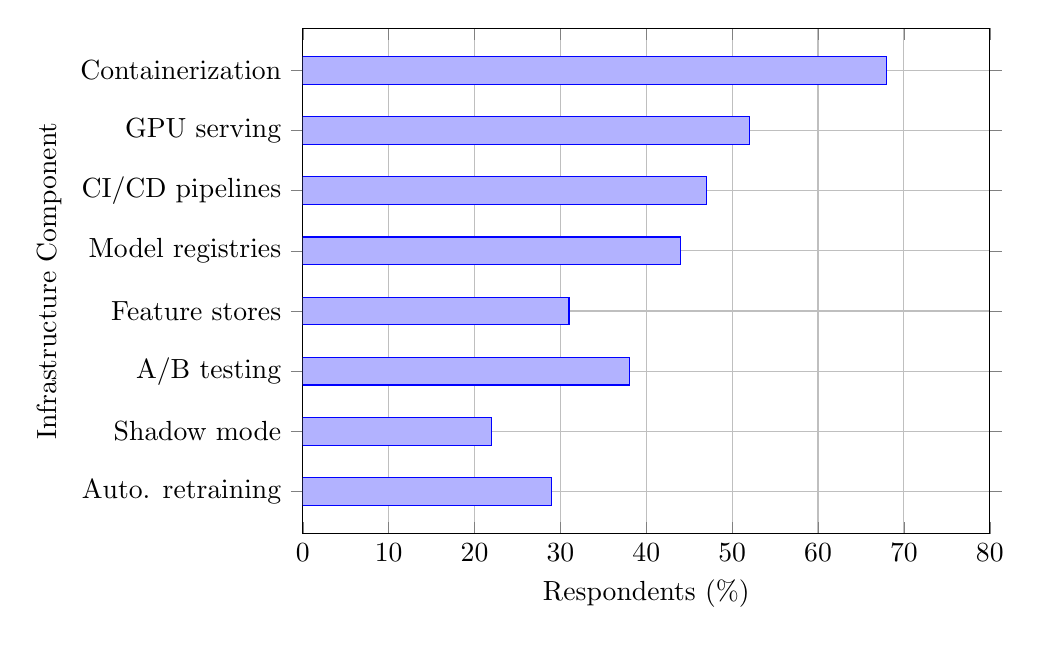
\begin{tikzpicture}
        \begin{axis}[
            xlabel={Respondents (\%)},
            ylabel={Infrastructure Component},
            xbar,
            width=0.85\textwidth,
            height=8cm,
            xmin=0, xmax=80,
            symbolic y coords={
                Auto. retraining, Shadow mode, A/B testing,
                Feature stores, Model registries, CI/CD pipelines,
                GPU serving, Containerization
            },
            ytick=data,
            bar width=10pt,
            grid=major,
        ]
        \addplot coordinates {
            (68,Containerization) (52,GPU serving) (47,CI/CD pipelines)
            (44,Model registries) (38,A/B testing) (31,Feature stores)
            (29,Auto. retraining) (22,Shadow mode)
        };
        \end{axis}
    \end{tikzpicture}
    \caption{Adoption rates of ML deployment infrastructure components.}
    \label{fig:deployment-bar}
\end{figure}

\subsection{Monitoring and Maintenance}

Post-deployment monitoring is critical for ML system reliability. Our
findings reveal:

\begin{itemize}
    \item 73\% of respondents monitor model prediction distributions,
          but only 38\% monitor for data drift using automated tools.
    \item 52\% have experienced at least one model performance degradation
          incident in the past year that went undetected for $>$ 1 week.
    \item Mean time to detect (MTTD) model failures: median 5 days
          (IQR: 2--14 days).
    \item Mean time to remediate (MTTR): median 3 days (IQR: 1--7 days).
\end{itemize}

\begin{table}[htbp]
    \centering
    \caption{Model monitoring practices and incident frequency.}
    \label{tab:monitoring}
    \begin{tabular}{@{}lc@{}}
        \toprule
        Metric & Value \\
        \midrule
        Monitor prediction distributions & 73\% \\
        Automated drift detection & 38\% \\
        Real-time performance dashboards & 45\% \\
        Automated alerting on degradation & 33\% \\
        Experienced undetected failure ($>$ 1 week) & 52\% \\
        Median MTTD for model failures & 5 days \\
        Median MTTR for model failures & 3 days \\
        \bottomrule
    \end{tabular}
\end{table}

\subsection{Organizational Factors}

Organizational support significantly impacts ML engineering maturity.

\begin{table}[htbp]
    \centering
    \caption{Organizational factors by ML maturity level.}
    \label{tab:org-factors}
    \begin{tabular}{@{}lcc@{}}
        \toprule
        Factor & High Maturity ($n = 412$) & Low Maturity ($n = 534$) \\
        \midrule
        Dedicated ML platform team & 78\% & 22\% \\
        ML-specific CI/CD investment & 82\% & 31\% \\
        Executive sponsorship for MLOps & 71\% & 28\% \\
        Cross-functional ML teams & 65\% & 34\% \\
        Regular model audits & 58\% & 19\% \\
        \bottomrule
    \end{tabular}
\end{table}

Organizations with high ML maturity (defined as scoring $\geq$ 4 on a
composite 5-point scale) are significantly more likely to have dedicated
platform teams ($\chi^2(1) = 289.4$, $p < .001$, Cramér's $V = .48$)
and executive sponsorship ($\chi^2(1) = 215.7$, $p < .001$).

\section{Statistical Analysis}
\label{sec:statistics}

\subsection{Predictors of ML Maturity}

A multiple logistic regression was performed to identify predictors of
high ML maturity. The model was statistically significant ($\chi^2(7) = 342.1$,
$p < .001$) and explained 38\% of the variance (Nagelkerke $R^2 = .38$).

\begin{table}[htbp]
    \centering
    \caption{Logistic regression: predictors of high ML maturity.}
    \label{tab:regression}
    \begin{tabular}{@{}lcccc@{}}
        \toprule
        Predictor & $B$ & SE & Odds Ratio & $p$ \\
        \midrule
        Team size $>$ 10 & 1.42 & 0.18 & 4.14 & $< .001$ \\
        ML platform team (yes) & 1.87 & 0.21 & 6.49 & $< .001$ \\
        Executive sponsorship & 1.23 & 0.19 & 3.42 & $< .001$ \\
        CI/CD for ML (yes) & 0.98 & 0.17 & 2.66 & $< .001$ \\
        Experience $>$ 5 years & 0.76 & 0.16 & 2.14 & $< .001$ \\
        Industry sector & 0.34 & 0.15 & 1.40 & .024 \\
        Country (US/EU vs.\ other) & 0.21 & 0.14 & 1.23 & .134 \\
        \bottomrule
    \end{tabular}
\end{table}

\section{Discussion}
\label{sec:discussion}

\subsection{Key Insights}

\begin{enumerate}
    \item \textbf{Deployment remains the bottleneck:} 67\% of respondents
          identified model deployment as the primary bottleneck, consistent
          with anecdotal reports from industry.
    \item \textbf{Testing maturity gaps:} Fairness and robustness testing
          are recognized as important but severely under-implemented.
    \item \textbf{Monitoring is reactive:} Most organizations monitor
          prediction outputs but lack automated drift detection, leading
          to extended periods of degraded model performance.
    \item \textbf{Organizational factors matter most:} The strongest
          predictors of ML maturity are organizational (platform teams,
          executive sponsorship) rather than technical.
\end{enumerate}

\subsection{Limitations}

\begin{itemize}
    \item Self-selection bias: respondents are likely more engaged with
          ML engineering topics than the general population.
    \item Predominantly English-speaking, Western sample limits
          generalizability.
    \item Cross-sectional design prevents causal inference about
          organizational factors.
\end{itemize}

\section{Recommendations}
\label{sec:recommendations}

Based on our findings, we recommend:
\begin{enumerate}
    \item Organizations should invest in dedicated ML platform teams as
          the single highest-impact intervention.
    \item CI/CD pipelines should be extended to cover data validation,
          model testing, and deployment automation.
    \item Fairness and robustness testing should be integrated into ML
          development workflows with automated tooling.
    \item Monitoring systems should shift from reactive (prediction
          logging) to proactive (automated drift detection and alerting).
\end{enumerate}

\bibliographystyle{plain}
\bibliography{references}

\end{document}
